\section{Virtual Analog Synthesis}

Der Begriff "Virtueller Analoger Synthese" wird verwendet, um die Echtzeit-Emulation des analogen Synthesizern der 60er und 70er Jahre zu beschreiben. Die Komplexität und die Ziele einer Emulation können variieren. Einige Emulationen gehen so weit, dass sie die tatsächlichen elektronischen Komponenten der Vintage-Synthese-Schaltungen zu simulieren, andere modellieren nur grob den Signalfluss.

Unabhängig von der Art der Emulation hat virtuell analoger Synthese zwei Probleme mit dem es sich Beschäftigen muss, Latenzzeit und Aliasing. Das Problem der Latenzzeit wurde bereits oben beschrieben. Die Verarbeitung wird eine Verzögerung des Signals erzeugen, die Komplexität der Verarbeitung kann die Verzögerung erhöhen oder mehr CPU-Zyklen verbrauchen. Aliasing ist ein hörbare Verzerrungen des Signals, welches durch Frequenzen verursacht werden die höher sind als die Abtastrate des Systems erlaubt.

Analog-Synthesizer verwenden üblicherweise Subtraktive Synthese. Ein oder mehrere Klangerzeuger ( Oszillatoren ) erzuegen Signale mit besondere harmonische Qualitäten. Diese Signale werden durch Filter geschickt, welche die Frequenzen aus dem Signal "Subtraktieren". Die Oszillatoren, Filter und Amplitude können moduliert werden. Abbildung~\ref{fig:synth_voice_block} ist ein einfaches Blockschaltbild eines typischen Subtraktive Synthesizer Stimme.

\begin{figure}[H]
    \centering
    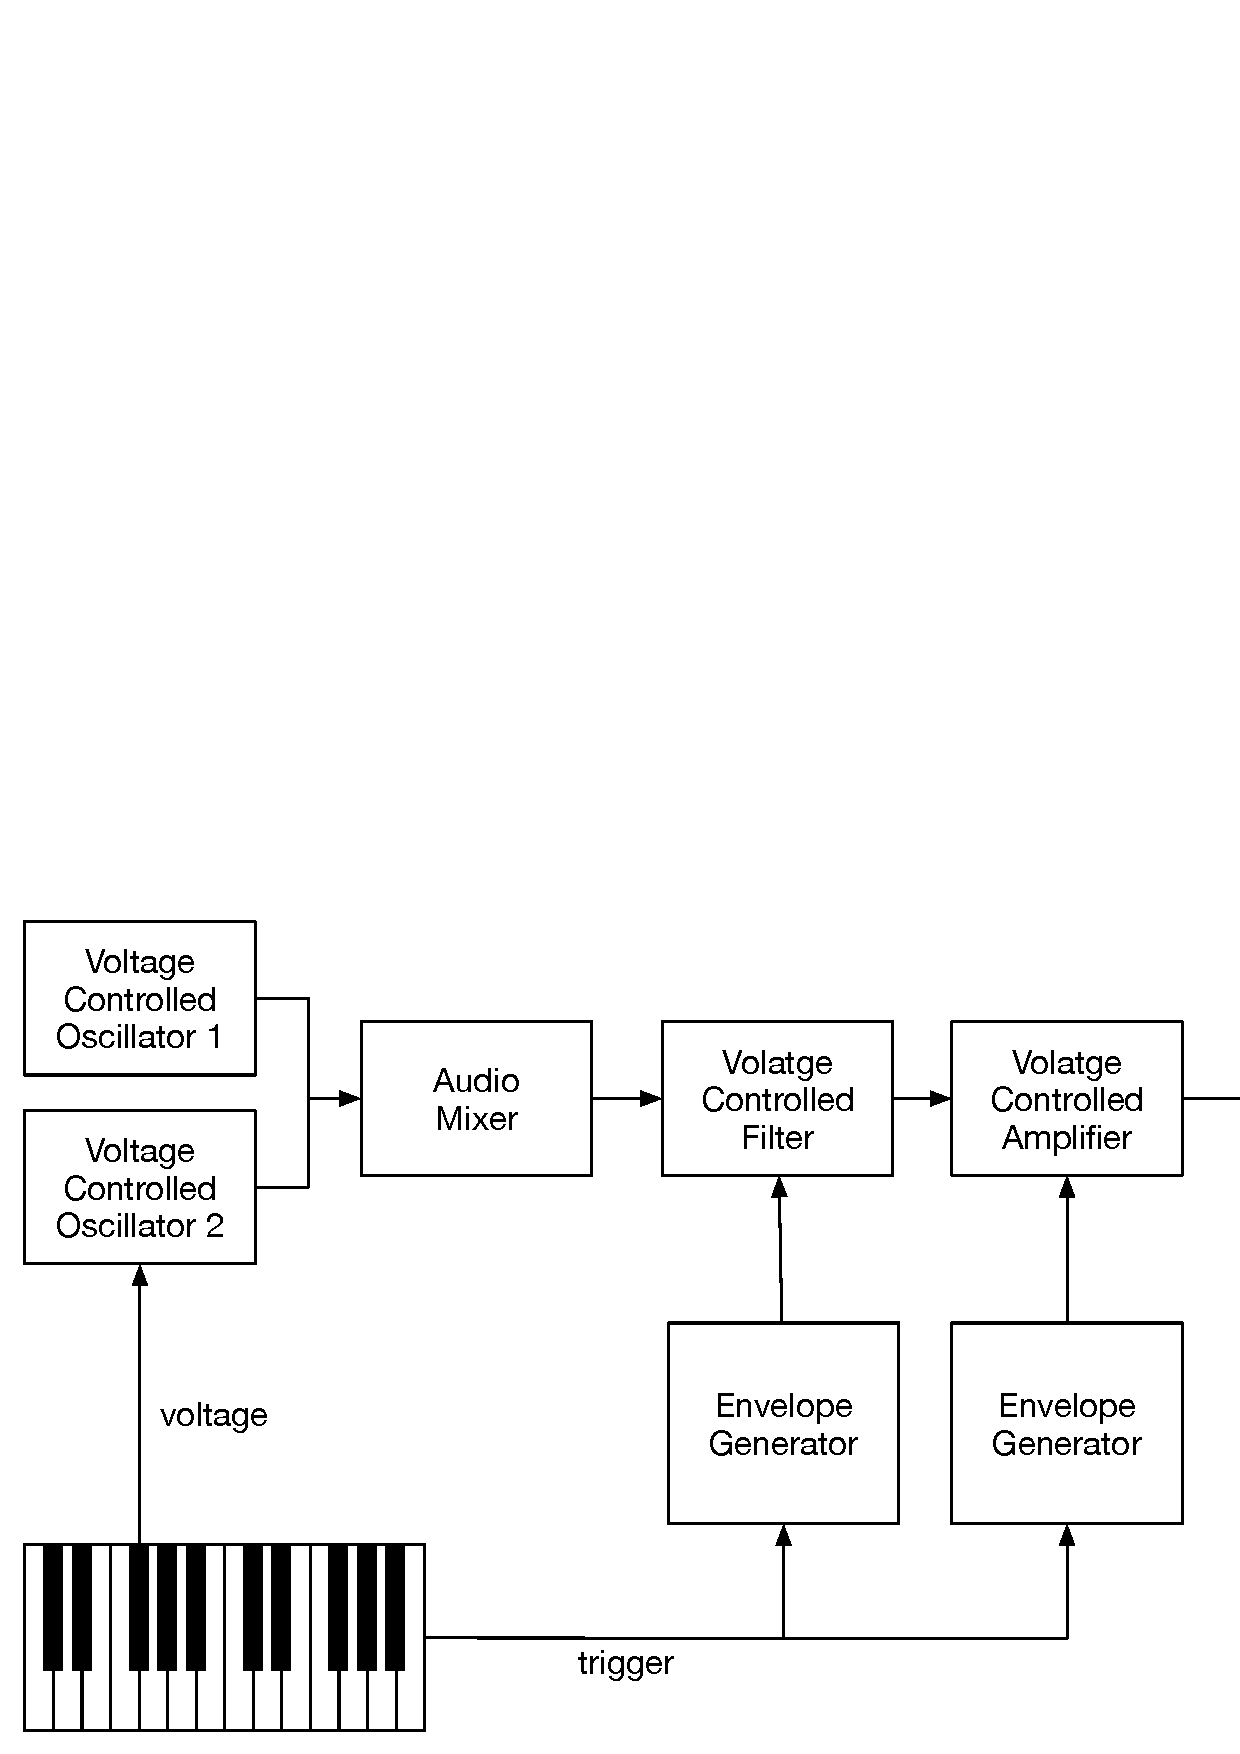
\includegraphics[width=\textwidth]{assets/synth_voice_block.pdf}
    \caption{Blockschaltbild eines Subtraktive Synthesizer Stimme}
    \label{fig:synth_voice_block}
\end{figure}

Die spannungsgesteuerte Oszillatoren (voltage controlled oscillators, VCO) erzeugen einfache Wellenformen in der Tonhöhe, die auf der Tastatur gespielt wird. Der Benutzer kann in der Regel zwischen einer Kombination aus Sägezahn, Rechteck oder Dreieckwellenform wählen. Die Frequenzen oder die Klangfarbe der Wellenformen können dann durch die folgenden Filter und Amplituden Blöcke moduliert werden.

Der erste Eindruck könnte sein, dass die Modellierung des Oszillators wäre einfach. Ein digital erzeugte Rechteck oder Sägezahn-Wellenform sollte trivial zu implementieren. Die 5 kHz Sägezahn Wellenform beispielsweise würde sich alle 8,82 Samples weiderholen bei einer Taktrate von 44,1 kHz. So würde die Wellenform linear von -1,0 bis 1,0 auf erhöhen, dann zurück auf -1.0 springen auf -1,0 und erneut anfangen. Was bedeutet aber 0,82 Samples in einer diskreten digitalen System? Abbildung ~\ref{fig:aliasing_sawtooth} veranschaulicht das Problem. Die linke Spalte zeigt einen Abschnitt eines idealisierten 5kHz Sägezahnwellenform und der entsprechenden Frequenzinhalt. Oberhalb der Grundfrequenz 5 kHz sind Oberwellen, die weit über 100 kHz hörbar sein werden. Die rechte Spalte zeigt den gleichen Abschnitt eines 5kHz Sägezahnwellenform in einem mit 44,1kHz getakteter diskreter Umgebung. Die Wellenform selbst ist verzerrt und die höheren Harmonischen sichtbar  vom 22,05 kHz Nyquist-Grenze nach unten reflektiert.

\begin{figure}[H]
    \centering
    \includegraphics[width=\textwidth]{plots/graphics/sawtooth.pdf}
    \caption{Ideal and Aliased 5kHz Sawtooth waveform}
    \label{fig:aliasing_sawtooth}
\end{figure}

Es gibt verschiedene Verfahren zur Beseitigung oder Verminderung von Aliasing. Die effektivste ist es, die Oberwellen mit einer Reihe von Sinus Wellen bis zu der Nyquist-Grenze oder die Hälfte der Abtastrate des Systems zu konstruieren, aber dies ist sehr rechenintensiv. Weniger CPU-intensive Strategien sind Oversampling, Bandlimiting oder andere Alias-Unterdrückungs Methoden\cite{virtual_analog_synthesis}.




